\documentclass[12pt]{beamer}
\usetheme{umbc4}
% \usetheme{Frankfurt}
% \usetheme{metropolis}
% \usetheme{moloch}

\usepackage{amsmath,amscd}
\usepackage{fontspec}
\usepackage{unicode-math}

%\metroset{background=dark}

% Set the slide body to black background with white text
\setbeamercolor{background canvas}{bg=black}
\setbeamercolor{normal text}{fg=white}
% Set the title bar to black background with white text
\setbeamercolor{frametitle}{bg=black, fg=white}
% Ensure other structural elements (bullets, etc.) are visible
\setbeamercolor{structure}{fg=white}

\setmainfont{Libertinus Serif}
\setsansfont{Libertinus Sans}
%\setmathfont{Libertinus Math}
\setmathfont{STIX Two Math}
%\setmathfont{Asana Math}

\newcommand{\nl}{\vspace*{1em}\\}
\newcommand{\vsp}{\vspace*{1em}}

\begin{document}

\begin{frame}\frametitle{Rewards, Returns and Episodes}
    If the sequence of rewards received after time step $t$ is $R_{t+1}, R_{t+2}, R_{t+3}, \ldots$,
    then the \textit{expected return}, $G_t$, is defined as the total reward from time $t$ onward:

    $$
        G_t = R_{t+1} + R_{t+2} + R_{t+3} + \ldots + R_T
    $$

    where $T$ is the time step when the episode ends.\nl
    Each episode is guaranteed to end in a finite number of steps, so $G_t$ is well-defined.\nl
    Each episode ends in a special state called the \textit{terminal state}.
\end{frame}


\begin{frame}\frametitle{Returns, Continuing Tasks, and Discounting}
    Some agent-environment interactions do not naturally break into episodes.\nl
    Tasks may go on forever, and we want to be able to talk about the return in these cases as well.\nl
    Agent tries to select actions so that the sum of the discounted rewards over
    the future is as large as possible.\nl
    $$
    \begin{array}{rll}
        G_t &=& R_{t+1} + \gamma R_{t+2} + \gamma^2 R_{t+3} + \ldots \nl
            &=& \sum\limits_{k=0}^{\infty} \gamma^k R_{t+k+1}
    \end{array}
    $$
    where $0 \le \gamma \le 1$ is called the \textit{discount rate}.
\end{frame}


\begin{frame}\frametitle{Discounted Rewards}
    A reward received $k$ time steps in the future is worth only $\gamma^{k-1}$ times its immediate value.\nl
    if $\gamma = 0$, the \textit{myopic} agent only cares about the immediate reward.\nl
    \begin{itemize}
        \item agent learns to choose actions that yield the highest immediate reward.
        \item agent chooses $A_t$ so as to maximize $R_{t+1}$.
    \end{itemize}
\end{frame}

\begin{frame}\frametitle{Farsighted Agent}
    As $\gamma$ approaches 1, the return objective takes future rewards into account more strongly.\nl
\end{frame}

\begin{frame}\frametitle{Returns in Successive Time Steps}
    $$
    \begin{array}{rll}
        G_t &=& R_{t+1} + \gamma R_{t+2} + \gamma^2 R_{t+3} + \ldots \nl
            &=& R_{t+1} + \gamma (R_{t+2} + \gamma R_{t+3} + \ldots) \nl
            &=& R_{t+1} + \gamma G_{t+1}
    \end{array}
    $$

    This works for all time steps $t < T$, if we define $G_T = 0$. \nl
    In the termination state, reward is zero.
\end{frame}



\begin{frame}\frametitle{Value Function of a State}
    $v_\pi$ is the value function of a state $s$ under a policy $\pi$.\nl
    A value function is the \textit{expected return} when starting from state
    $s$ and following policy $\pi$ thereafter.\nl

    $$
    \begin{array}{rll}
        v_\pi(s) &=& \mathbb{E}_\pi [G_{t} \,|\, S_t = s]\nl
            & = & \mathbb{E}_\pi \left[\, \sum\limits_{k=0}^{\infty} \gamma^{k} R_{t+k+1} \,\middle|\, S_t = s \,\right]\!,\,\mathrm{for \ all \ } s \in \mathcal{S}  \nl
    \end{array}
    $$
    \vsp
    In an MDP, this is true for all states $s$ in the state space $\mathcal{S}$.

\end{frame}


\begin{frame}\frametitle{Bellman Equation for Value Function $v_\pi$}
    A \textit{Policy} $\pi$ is a mapping from states to probabilities of selecting each possible action.\nl

    If the agent is following policy $\pi$ at time $t$, then $\pi(a|s)$ is the probability that $A_t = a$ when $S_t = s$.\nl

    The $\mid$ operator defines a probability distribution over $a \in \mathcal{A}(s)$ for each $s \in \mathcal{S}$.\nl

\end{frame}

\begin{frame}\frametitle{Bellman Equation for Value Function $v_\pi$}
    $$
    \noindent\begin{array}{lll}
        v_\pi(s) &=& \mathbb{E}_\pi [G_{t} \,|\, S_t = s]\nl
            &=&  \mathbb{E}_\pi [R_{t+1} + \gamma G_{t+1} \,|\, S_t = s] \nl
    \end{array}
    $$

    The expectation is over the joint randomness of the action chosen by $\pi$, the next state, and the next reward.
\end{frame}


\begin{frame}\frametitle{Bellman Equation for Value Function $v_\pi$}
    $$
    \begin{array}{lll}
        v_\pi(s) &=& \mathbb{E}_\pi [G_{t} \,|\, S_t = s]\nl
            &=&  \mathbb{E}_\pi [R_{t+1} + \gamma G_{t+1} \,|\, S_t = s] \nl
    \end{array}
    $$

    Actions under $\pi$ \vspace*{2mm}\\
    \hspace*{5em}$\sum\limits_{a} \pi(a|s)$\nl

    Next states and rewards \vspace{2mm}\\
    \hspace*{5em}$\sum\limits_{s'} \sum\limits_{r} p(s', r | s, a)$\nl

    Reward + Discounted reward\vspace*{2mm}\\
    \hspace*{5em}$\bigg[\,r + \gamma \mathbb{E}_\pi \big[\,G_{t+1} \mid S_{t+1} = s'\,\big] \bigg]$
\end{frame}


\begin{frame}\frametitle{Bellman Equation for Value Function $v_\pi$}
    $$
    \hspace*{-8pt}\begin{array}{lll}
        v_\pi(s) &=& \mathbb{E}_\pi [G_{t} \,|\, S_t = s]\nl
            &=&  \mathbb{E}_\pi [R_{t+1} + \gamma G_{t+1} \,|\, S_t = s] \nl
            &=&  \sum\limits_{a} \pi(a|s) \sum\limits_{s'} \sum\limits_{r} p(s', r | s, a) \,\bigg[\,r + \gamma\,\mathbb{E}_\pi \big[\,G_{t+1} \mid S_{t+1} = s'\,\big] \bigg]\,  \nl
            &=&  \sum\limits_{a} \pi(a|s) \sum\limits_{s', r} p(s', r | s, a) \,\bigg[\,r + \gamma\, v_\pi(s') \bigg], \ \text{for all } s \in \mathcal{S}  \nl
    \end{array}
    $$
\end{frame}

\begin{frame}\frametitle{Backup Diagram}
    Each open circle, $\circ$, represents a state. \nl
    Each solid circle, $\bullet$, represents a state-action pair. \nl
    Starting from state $s$, the agent can take action $a$ with probability $\pi(a|s)$.\nl
    \begin{figure}[htbp]
        \centering
        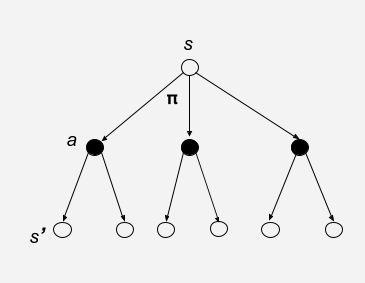
\includegraphics[width=0.5\textwidth]{backup_diagram.png}
    \end{figure}
\end{frame}

\begin{frame}\frametitle{Backup Diagram}
    \begin{minipage}{0.54\textwidth}
        Backup operations transfer value information \textit{back} to a state from the successor states.\nl
        State nodes need not represent distinct states. \nl
        \textit{A state may be its own successor.}
    \end{minipage}\hfill
    \begin{minipage}{0.44\textwidth}
        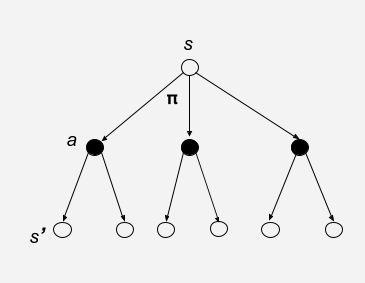
\includegraphics[width=5cm, height=4cm]{./backup_diagram.png}
    \end{minipage}
\end{frame}

\end{document}
